\section{Scenario Introduction}\label{introduction:scenario}
% Scenario introduction
A marathon runner is racing a track shaped as shown in figure 1, while equipped with sensor node A. The sensor node is broadcasting four packages per second tracking the runner’s pulse history. The level of details in the tracking package defines the number of marathons possible for the runner to run before a new battery is required. At one time the track was closed, resulting in the runner racing around the building of her workplace.

%\begin{figure}[H]
%	\centering
%	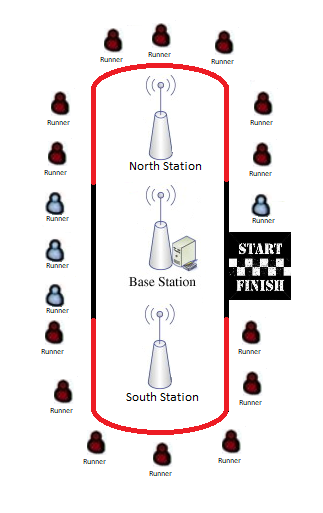
\includegraphics[width=0.8\linewidth]{scenarioIntroduction}
%	\caption{A marathon runner "node A" is racing around a track, while transmitting pulse information to the base station. In the red northern territory, node A transmits to the north station which relays the message to the base station. Likewise, at the southern station.}
%	\label{fig:scenarioIntroduction}
%\end{figure}

\begin{figure}[h]
	\centering
	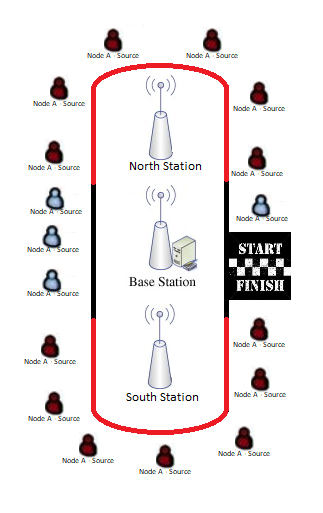
\includegraphics[width=0.8\linewidth]{introduction/scenario/fig/scenarioIntroduction.png}
	\caption{A marathon runner "node A" is racing around a track, while transmitting pulse information to the base station. In the red northern territory, node A transmits to the north station which relays the message to the base station. Likewise, at the southern station.}
	\label{fig:scenarioIntroduction}
\end{figure}


\section{Protocol introduction “To hop or not to hop”}
Node A will be broadcasting with a packet size of 128 Bytes. The base station will collect the data from node A when in range and save the data. The North station will, when in range and the base station is out of range, receive and relay the message to the base station. The same scenario will happen at the south station. Time Synchronization, Localization and Scalability will be considered regarding the protocol design. Each and combined scenarios will be evaluated in relation to signal strength relative to power consumption and data reliability. 

\subsection{Source: Node A}
Source node A will be transmitting at a periodic transmission rate. Different levels of power consumption will be determined by the chosen protocol, but, in any case, the power consumption will be considered, over a period of one second, constant. The less power consumption of node A will give longer individual lifetime and runtime for the runner, but low signal strength of node A might not give a lowest possible system power consumption. Depending on the needed quality of the received package, e.g. -3db, a cut of distance will be calculated and measured. Distance measuring will be limited by interference providing a need for a scalable transfer function estimate and an average over multiple measurements. Life time of node A will be considered when half of the battery capacity is used.

\subsection{Sink and Source: North and South Station}
Idle time, receiving and transmitting power consumption will be calculated and measure. When out of range the “pole” stations will go to an idle state to save power. When in transmitting mode different measurements will be conducted depending on the chosen protocol. E.g. firm or no handshakes between pole station and base station will be measured leading to different possible distances between jumps.

\subsection{Sink: Base Station}
The required detail of information needed to give a good user estimate will raise the question of acceptable package loss. Signal strength, package frequency, package loss vs reliability from both pole stations and source will determine the power consumption of the base station and the system. The base station will never be in idle state and it must be able to reach pole station resulting in the highest cost function of the system. 

\subsection{Test Scenario}
On the datasheet of the TelosB, the current draw when on receive mode is stated to be $23mA$. However since the transmit power is not given in the datasheet, testing is needed to gain further knowledge of how much power is used when sending and receiving data between nodes. The test data will be used to conduct different scenarios of the main scenario in which the end result will be the lifetime of the WSN and the minimum power consumption of the WSN. The conclusion will then be used together with the conclusion of the signal strength testing, to conduct the best scenarios for when to hop or not to hop.